\documentclass[12pt,twocolumn]{article}

%packages
\usepackage{graphicx}
\usepackage{array}
\usepackage[utf8]{inputenc}
\usepackage{float}     
\usepackage{wrapfig}
\usepackage{caption}

%include paths
\graphicspath{{./Images/}}

%extras
\setlength{\parindent}{8ex}

%Title information
\title{Digital Alarm Clock}

%\subtitle{semester 2 \\ Laboratory Practice-I}
\author{Group-22\thanks{Supervisors : Mr.Pramitha Theekshana Mukuthukudaarachchi, Mr.Pasan Dissanayake}}
\date{\today}

\begin{document}


\begin{titlepage}

    \maketitle
    
\includegraphics[scale=0.5]{mora}
    \centering

    \begin{center}
        Department of Electronic $\&$ Telecommunication Engineering\\University of Moratuwa\\
    \end{center}


    \begin{center}
        \begin{tabular}{  m{10em}  m{5em} }
            S.Sanjith  & 190562G \\
            T.Sajeepan & 190539T \\
            K.G.C.P.Sandaruwan  & 190557V \\
            G.S.M.U.K.Samarakoon & 190543B \\
        \end{tabular}
    \end{center}


\end{titlepage}

\newpage
\onecolumn
\tableofcontents
\begin{center}
    This report is submitted as a partial fulfillment of module EN1093.
\end{center}


\newpage
\twocolumn
\begin{abstract}
    Time is so precious and waking up at the desired time will help to make it through a
    busy day easily. Therefore, an alarm clock is a necessary item for anyone nowadays. 
    
    We have developed a simple alarm clock that displays user modifiable time and have the ability
    to manage up to six alarms in real-time, using ATmega328p as the brain and some other inexpensive electronic components.

    Beyond the simple design, We experimented with PCB designing, various aspects of enclosure
    design and other aesthetic aspects which would stand behind our product to make it 
    commercially successful.
\end{abstract}


\section{Introduction}
This paper discusses the complete design and fabrication of a digital alarm clock that can detect alarm
time by comparing the current time with stored alarm times. The output of the device when an alarm is 
active is given by a speaker and also the stored name of the alarm is indicated on the display. 

Considering the memory requirements and IO pins, ATmega328P is decided as the brain of this device. 
For the purpose of taking outputs, display  LCD $16\times2$, RTC DS3232 module, and a speaker are used. Other than these 
amplifying circuits, power regulation circuits are also implemented.

The communication between the LCD screen and ATmega328P was established with the help of digital 
communication. RTC module and chip communication is made in a serial manner using I2C communication. 
And digital pins are also used to detect the keypress in this device.

Most part of this paper discusses virtual stimulation of the device rather than real implementation. 
For programming the ATmega 328P, microchip studio and vs code platforms were used. PCB designing was 
made on Altium and Solidworks software used in Enclosure design. The final demonstration of the device
was done with the help of the Proteus platform. Additionally, miro and whiteboard apps were used to 
discuss and brainstorm ideas.


\section{Methodology}
    \subsection{Micro Product}
In the early stage, the project was divided into four subparts. \textbf{Key Input} is intended to get hands-on
experience with relating Keypad, microcontroller, power regulator and LEDs,  \textbf{Output} to experience with
linking LCD, microcontroller, power regulator and buttons, \textbf{Alarm Timing} to work with RTC,
microcontroller, LEDs and buttons, and \textbf{Audio Output} to play with Buzzer/speaker, microcontroller,
buttons, and a speaker. Proteus simulations were done for each sub-system. Separate PCB designs and
enclosure designs were created, and final micro products were demonstrated for the second evaluation.
Experiences gained from all four subsystems were combined when working with the final stage product.  



    \subsection{Operational Requirements}
Starting with requirements the following functionalities were expected to include in the final 
implementation.
\begin{enumerate}
    \item Set Current Date and Time.
    \item List the existing alarm
    \item Set a new alarm
    \item Edit or Delete alarm
    \item Select an alarm Tone
    \item Factory Reset
\end{enumerate}
This document explains about a sample alarm clock with same kind of functionalities ~\cite{sandilya2018design}


    \subsection{Main Component Selection}
The clock design consists Atmega328PU microcontroller as main chip, LCD16x2 and 
RTC-DS3232 as main components to achieve the functionality. 

        \subsubsection{ATmega328P}

\begin{wrapfigure}{l}{0.2\textwidth}
    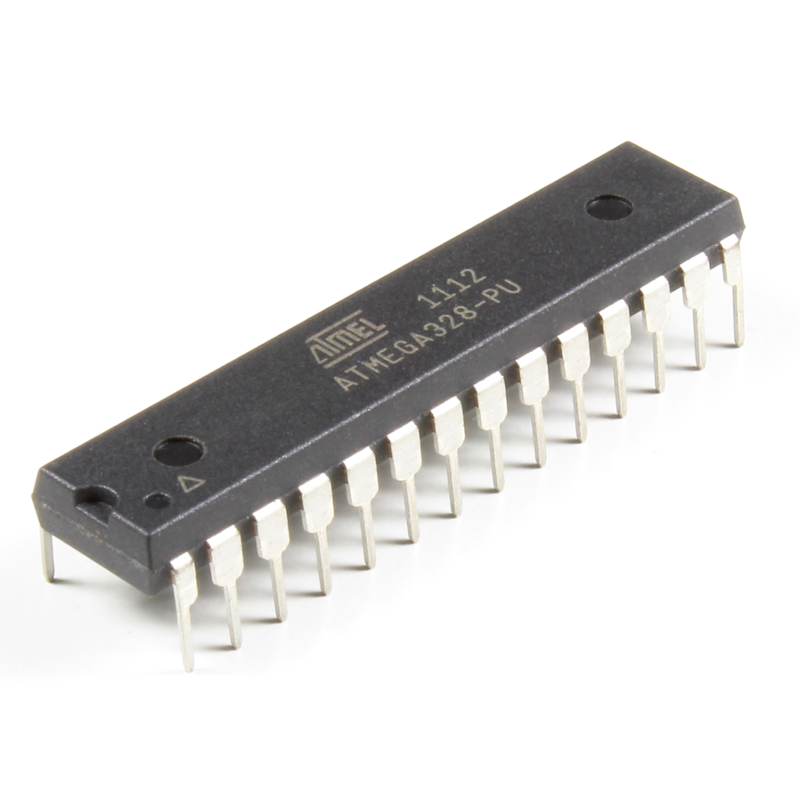
\includegraphics[width=0.2\textwidth]{chip}
\end{wrapfigure}

Design of the digital alarm clock requires more than fifteen digital Input-Output pins to establish
proper communication between components of the device. More than one PWM channel is expected to 
produce pulse waves for tones. Inside memory of the chip device has to store program files,
tones, and alarm parameters.

Considering requirements and effective solutions ATmega328P is concluded as the main chip brain of the 
device. It provides a total of twenty-three I/O pins where six of which could be used as PWM channels.

It contains a total of 32Kb program memory which even allows storing tones in the hardcoded manner and
1Kb EEPROM for storing parameters even during powerfailures. The power requirement range of the chip 
from $1.8V\to5.5V$ and other mentioned features perfectly matches the needs of the product. 
A very helpful referece about ATmega328P is~\cite{widadi2020atmega328p}  

        \subsubsection{16x2 LCD Display}
        
\begin{wrapfigure}{r}{0.2\textwidth}
    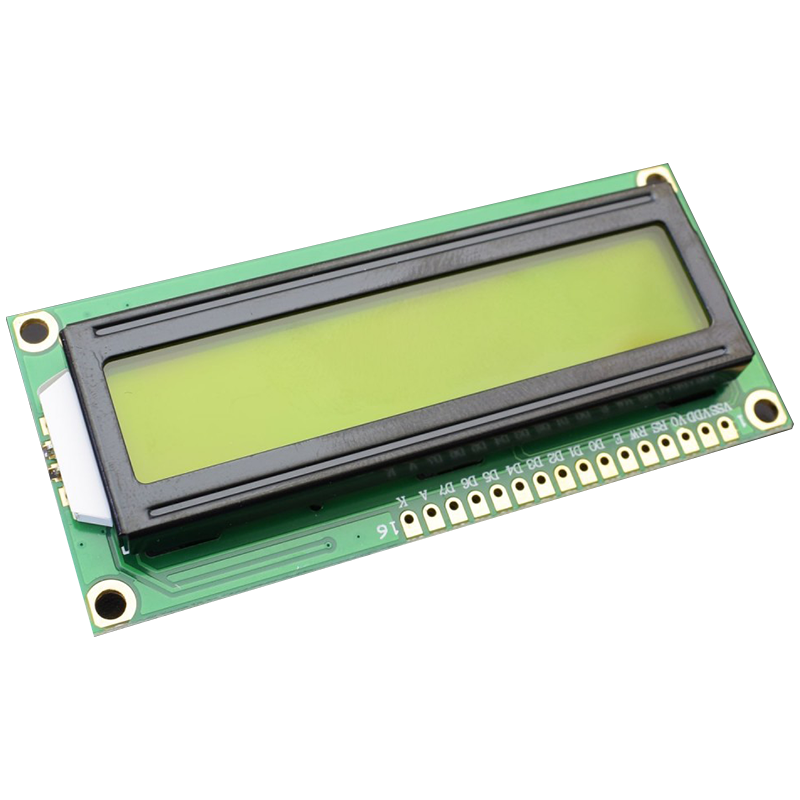
\includegraphics[width=0.2\textwidth]{display}
\end{wrapfigure}


The display is the main interface of the design which creates an interactive environment with the 
user to manage the functionalities of the clock to give inputs for alarm and time parameters.
Other than setting up the device normal clock function of displaying date and time was expected
as the default output from the display. It was expected to have a maximum of 30 characters in the
display.

Features of LCD16X2 Display such as character availability, power range(4.5V $\to$ 5.5V) 
make it feel like a component perfectly tailored for clock design. In addition, the screen allows
the user to adjust contrast and backlight brightness which add up to improvise the quality of design.


        \subsubsection{DS3232 RTC Module}
Keeping track of time and date accurately is the most important thing in a clock design. Although 
ATmega328 contains two 8-bit timers which are capable of tracking time, it is not accurate because 
power failure results in resetting of time and date. Due to that battery-backed DS3232 RTC module is 
used to keep track of time.

The module is more accurate than other available RTC modules like DS1307. It provides a 56Byte 
register for tracking and holding the time. The general-purpose RAM is provided with unlimited writes 
which allow the user to carry out read and write operations through I2C communication with the ATmega. 

        \subsubsection{Buttons and Switches}
Although a 3x4  keypad module is used for micro product design for the sake of simplicity in the 
final design only push-buttons are placed. To give a really nice user-friendly experience two 
keys are used for select and return purposes and another two for scrolling and one big button to 
snooze the alarm. In the final implementation, a hidden reset button is also included in order to 
allow the user to reset the device in a protected manner.


        \subsubsection{Speaker}
A small  4ohm speaker is included in the clock design to output the alarm tone sound. Since generating 
a high pulse by having a direct connection between ATmega and speaker results in high pulse feedbacks 
which may harm the chip, an amplifier circuit is also implemented in between the speaker and chip.

LM386 amplifier with amplification factor set to hundred is used for this purpose. Input power of 
amplifying circuit passed through a potentiometer to provide facility to manage alarm sound in the 
design.

    \subsection{Design Flow}
In the final design of the alarm clock user is allowed to create a maximum of six alarms with three 
alarm tone choices at the same item. Alarms are allowed to be repeated according to user choice. 
A reminder about the alarm is indicated in the display to remind the user about 
the alarm state. In case the user screwed things up, a safer reset button was also implemented to 
allow the user to reset the device more safely.

Considering the proper implementation of the design, the work was divided between members according 
to the following categories...
\begin{itemize}
 \item Main algorithm and Code development.
 \item Designing the final circuit sketch and PCB.
 \item Designing the enclosure.
 \item Combining the micro products files and developing firmwire libraries.
\end{itemize}

    \subsection{Parameters}
The structural data type is used for storing and using alarm and RTC parameters effectively. 
Every alarm has a separate name, time, date, recurring state, and alarm state values.
In order to easily modify and compare alarm parameters rather than storing real parametric values, 
they are stored in separate arrays and their appropriate indexes are indicated as alarms parameters. 

To help the functionality of the clock while creating and modifying alarms one integer parameter
is maintained to keep track of true alarms count. To efficiently check for alarm time parametric
reference for the first is alarm is maintained and updated at every modification in any of the
alarms. Other than this alarm sort function is also responsible to manage the date of the alarm
automatically according to the need.

    \subsection{Functional Units}
In order to understand the functioning of the clock, it can be viewed to function under three main 
functional units. Normally clock-works under-\textbf{display time} functional unit. Once an alarm 
time is detected to match with the current time \textbf{alarm time} comes under operation. 
Otherwise, pressing select key once leads to the \textbf{main menu}.

        \subsubsection{DisplayTime}
Get the current time and date from the RTC module and display it according to the required format 
after checking the value of the clock mode(zero stands for 24-Hour mode). In addition, here to indicate
any of the alarms is in on state a $"*"$ sign is displayed on the bottom right corner of the display according 
to whether the value for true alarms counts is greater than zero.

        \subsubsection{Alarm Ringing}
When the operational pointer enters the alarm time unit, the speaker starts to sound.
The commands to the speaker from ATmega are handled by storing tones in a format such 
that they are a collection of calling of different frequencies for a certain duration of 
time. Tones are named and stored appropriately to give the order and duration for frequencies 
in a sequential manner inside program memory rather than in ROM due to memory insufficiency. 

Since the duration of particular frequency calls is very small, checking for a keypress in 
between each frequency calling allows the device to ideally have the operation of interrupting 
alarm possible. 
        
Once the alarm is interrupted with return key alarm parameters are changed in accordance 
with the recurring state and the alarm list is sorted to return the position of the first alarm.
Snooze interruption also leads to same kind of operation except for the fact that alarm time gets
incremented with the snooze time.
        \subsubsection{Main Menu}
Operations required to change all the parameters of RTC and alarms go here. A hierarchical order
is maintained to go between options. An infinite loop is implemented in each hierarchy to keep the
current position of the operational pointer inside the appropriate hierarchy until necessary operations
are done. In addition, an integer parameter called level is maintained to keep track of order of the
hierarchy of operational pointer. Another integer array of length maximum level is maintained to keep track
of the item into which operational pointer is in under each order of hierarchy.

In any possible case, the select key increases the order of hierarchy of a particular unit by
increamenting the value of tracker, level value. Return key brings back to the previous order
of hierarchy. Mod operation during addition and subtraction of one to item value during navigation
allows maintaining a circular scrolling through available options of a particular hierarchy.

    \subsection{PCB Design}
Altium Designer is used to designing the PCB. The size of the PCB is kept as small as possible to
reduce the cost of fabrication. Dimensions of the PCB are set to 45 mm X 65 mm.

In the power regulation part, the 7805 voltage regulator IC is used to supply 5V stable power and
the Schottky diode is used to avoid damaging the circuit if battery terminals are accidentally
interchanged. Headers are used to connect all the modules and some of the other components to the
main PCB. This made repairing possible at a low cost. 
    
In the backside of the PCB, two potentiometers are mounted to control the contrast of LCD and volume
of the speaker. Five pushbuttons are also mounted on that side of the PCB to fit them on the backside
of the enclosure. Refer to the schematic and 3D model of PCB in the appendix.

    \subsection{Enclosure Design}

\begin{wrapfigure}{r}{0.2\textwidth}     %Here we specify the width of the image
    \centering                        % Here center of alocated space
    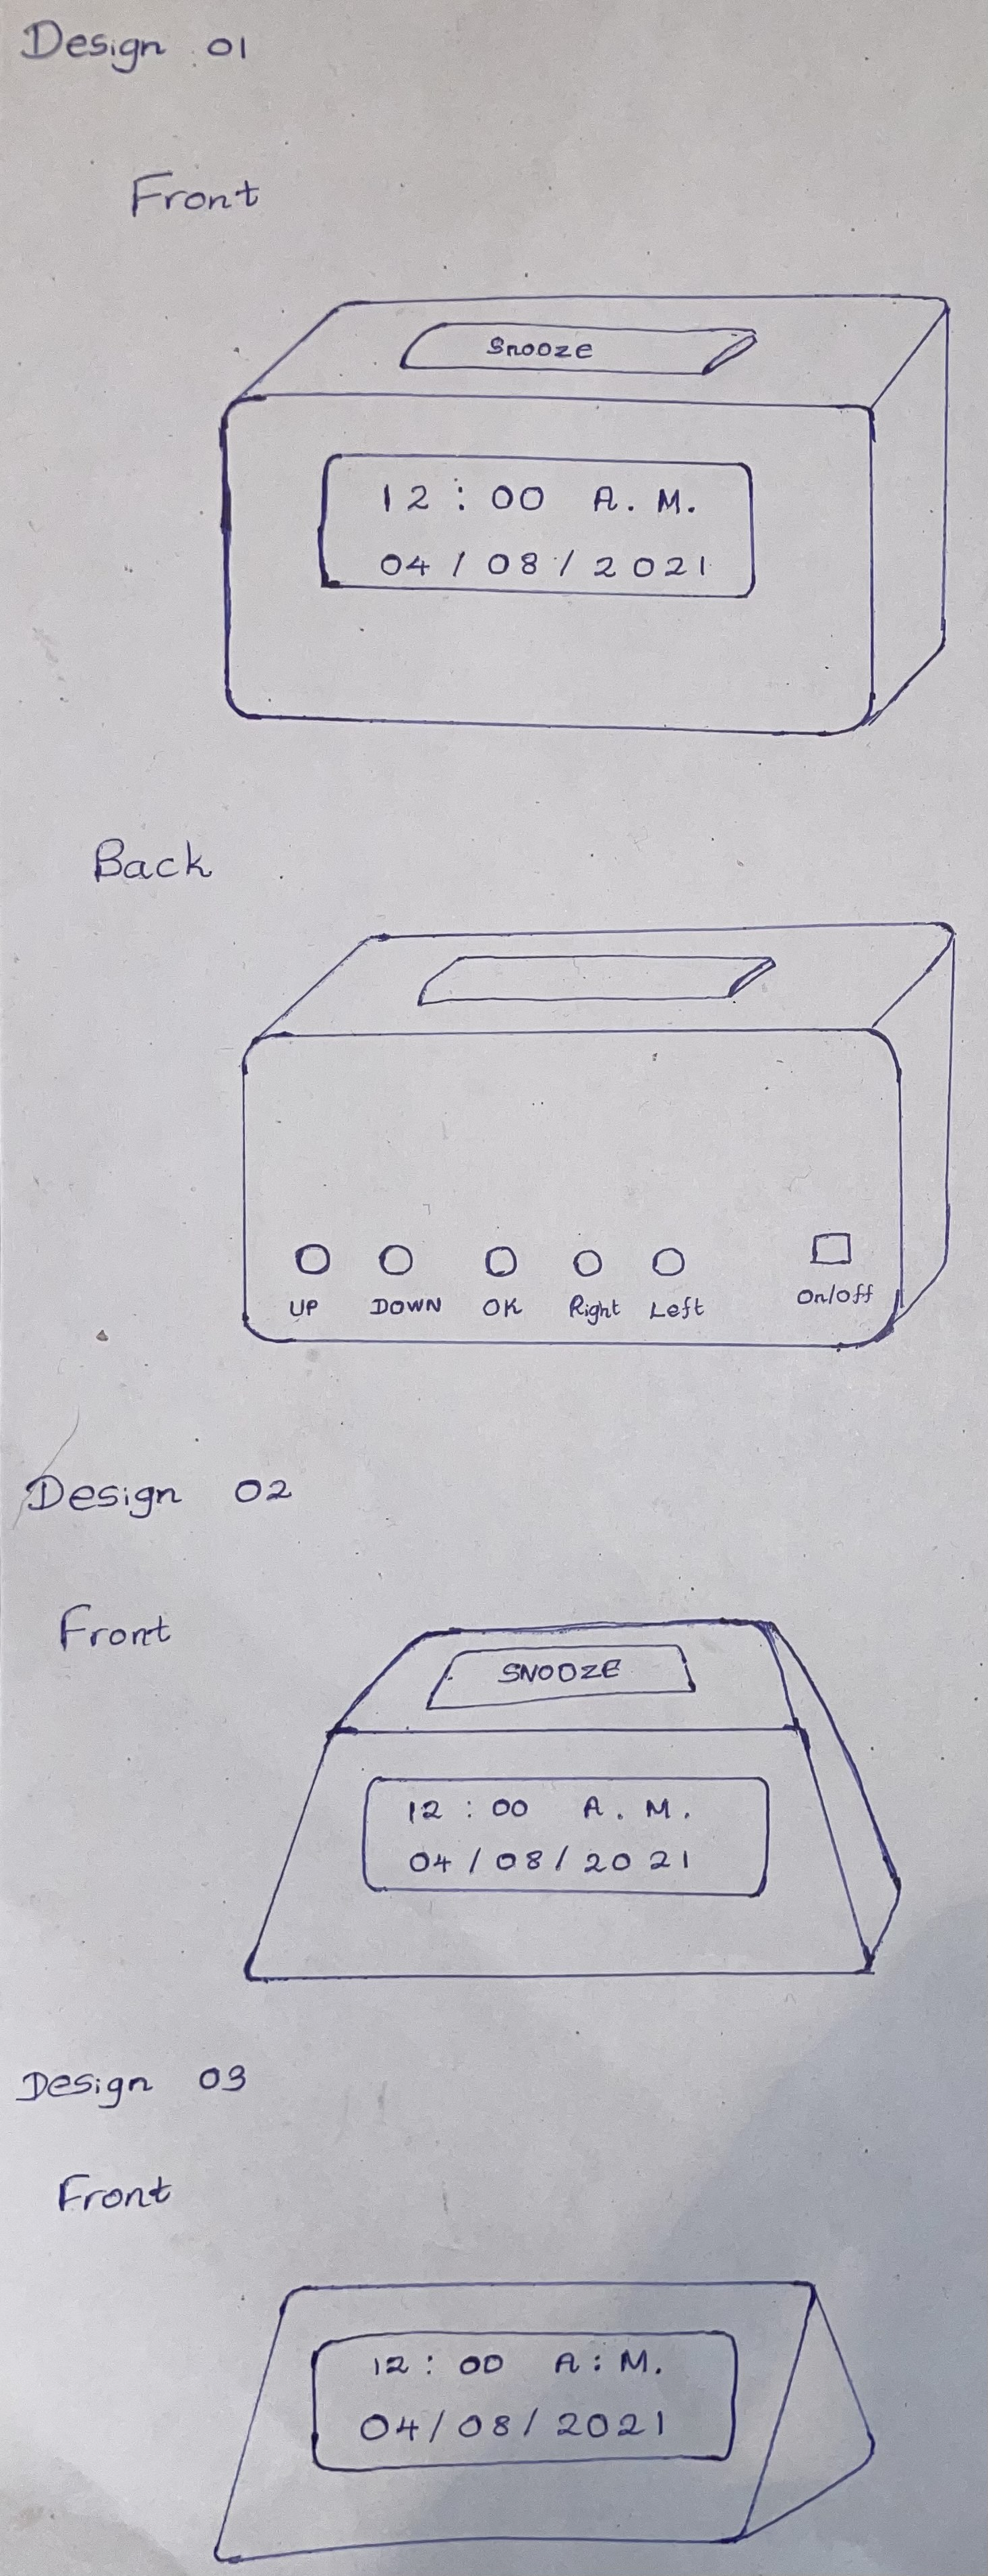
\includegraphics[width=0.2\textwidth]{drawing}
    \caption*{Hand Sketches} 
\end{wrapfigure}
The enclosure design of the alarm clock has been designed with a very simple exterior to be handled
easily by any person after looking into some designs in the market. In the early stage, few designs
were hand sketched and chose according to the feedback from random people. Some modifications were
also added to the initial sketch. Then, moved on the computer-aided design, and the software called
Solidworks Educational Edition was used for that purpose. 
    
In the front, there is nothing but the LCD screen because it is desired not to distract the user by
keeping other things, and in the back, all the buttons have been provided including five push buttons
and two rotating buttons. Access to the battery compartment and the speaker cutout is also in the back
of the enclosure. At the top, there is a big snooze button, an indicating led, and the reset button.
The dimensions of this box-shaped enclosure are 50mm x 76mm x 125mm. 
    
After getting the dimensions, the size of the PCB is decided and where should the buttons be contained.
The speaker is mounted under the PCB and it also can be replaceable and the RTC module is mounted on
the side to the PCB. The enclosure consists of 6 mounting bosses to assemble the front and back parts.
\section{Results}
On turning the device ON, the user will see a welcome message displayed on the LCD. Following that 
current time and date are displayed in the format of $HH:MM,\ DD:MM:YYYY$. Normally time is showed 
in 12 hours format. It can be changed to 24 hours format according to preference under-clock mode 
option in setup. 

The presence of the “*” symbol in the bottom right corner indicates one or more alarms in the active
stage. Users can go to the setting menu, by pressing the select option and proceed with the next 
operation in a normal manner. An indicator LED will light up to indicate the clock is in setting 
mode once the operational pointer enters the menu. 

Users can return to the previous operation by aborting the current operation with the press of the 
return button. Inside setup, the device is designed to consider times as in a 24- hour format.\par when
the user enters to edit alarm option and if there is no alarm in active mode it will automatically 
navigate create alarm procedure. Users can set up to five alarms. It can be given any name, tone, 
and repeat mode simply by looking at options on the screen.

While alarm ringing users have two options to interrupt the alarm in the middle, stop alarm and snooze 
alarm. If the user snoozes the alarm with snooze button it will stop ringing and reactivate after five
minutes and this will continues until user stop the alarm. Stopping the alarm will reactivate
alarm according to the specified repeat mode parameter.
\onecolumn
\begin{center}
    \begin{figure}[h]
    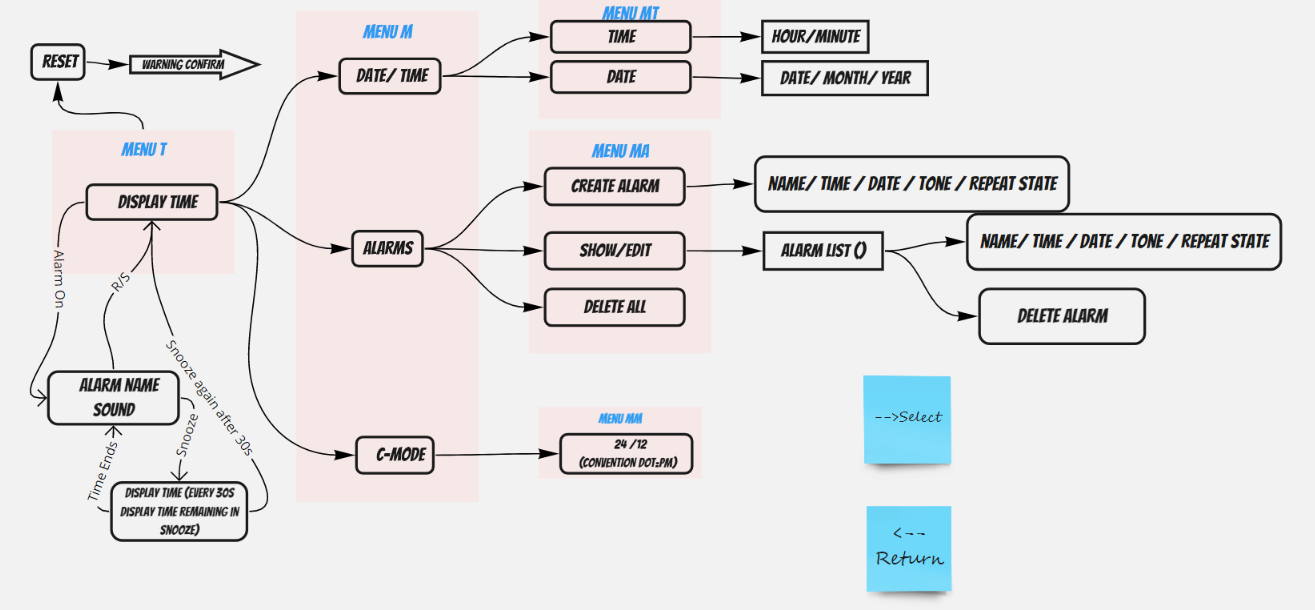
\includegraphics[width=\textwidth]{flow}
    \caption{This is the predefined functional flow of the product.}
    \end{figure}
\end{center}


\begin{center}
    \begin{figure}[h]
    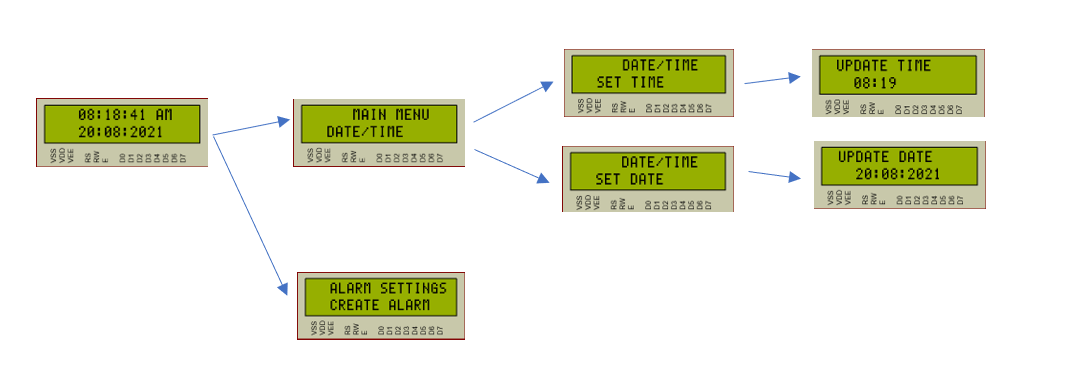
\includegraphics[width=0.73\textwidth]{flow2}
    \caption{This is the Output from LCD.}
    \end{figure}
\end{center}


\twocolumn


\section{Discussion}
    \subsection{Storing Alarm Tones}
In earlier, while designing and developing the algorithm five alarm tones are included for the alarm 
tone option. But while compiling the code due to the lack of memory compiler could include only three
tones due to Atmega328PU contains only limited storage of 32Kb Flash program memory. The tones are 
stored in an array sequence of notes with duration. 

Due to the big size of the array even one tone is not fit for EEPROM. Code files other than tone file
takes more than half of the program memory. Therefore, We are only able to include three tones. 
Even-though considering options with more memory allows the device to have more tones, but it results 
in exceeding the cost approximation of the device which makes the product inconsistent. 
    
    \subsection{Bouncing of Keys}
In the designing process, one keypress is detected as multiple presses of the same key due to the 
input value hold in the register for some time. This leads to iterations of the corresponding function 
several times. In order to get rid of this issue in the product, bouncing delay is introduced into the 
key handling algorithm. 

The delay time was checked in between the values 300$\to$1000 milliseconds. With the experiment, it is
decided to have 700 milliseconds for SELECT and RETURN buttons and 500 milliseconds for UP and DOWN 
buttons as bouncing time. Even after that bouncing is detected sometimes. It may be an environmental 
issue. 

    \subsection{Alarm-Handling in Setup}
when the user is in the setting menu if the alarm time arrives, the alarm does not ring and after 
escaping from the setting menu it only rings if alarm time and current time are exactly the same 
otherwise it will automatically be reactivated for the next day. This is because the designed algorithm
handles only the sequential operation and ATmega328p does not support parallel processing.

\section{Acknowledgements}
We, as a team, sincerely thank our supervisors, Mr. Pramitha Muthukudaarachchi and
Mr. Pasan Dissanayake for their guidance, patience, and for the valuable feedback they
gave us through progress meetings, without which this project would not have been what it is today...

\bibliographystyle{plain}
\bibliography{./bibliography}

\newpage
\onecolumn
\appendix
\section{PCB Schematic Diagram}

\begin{center}
\begin{figure}[h]
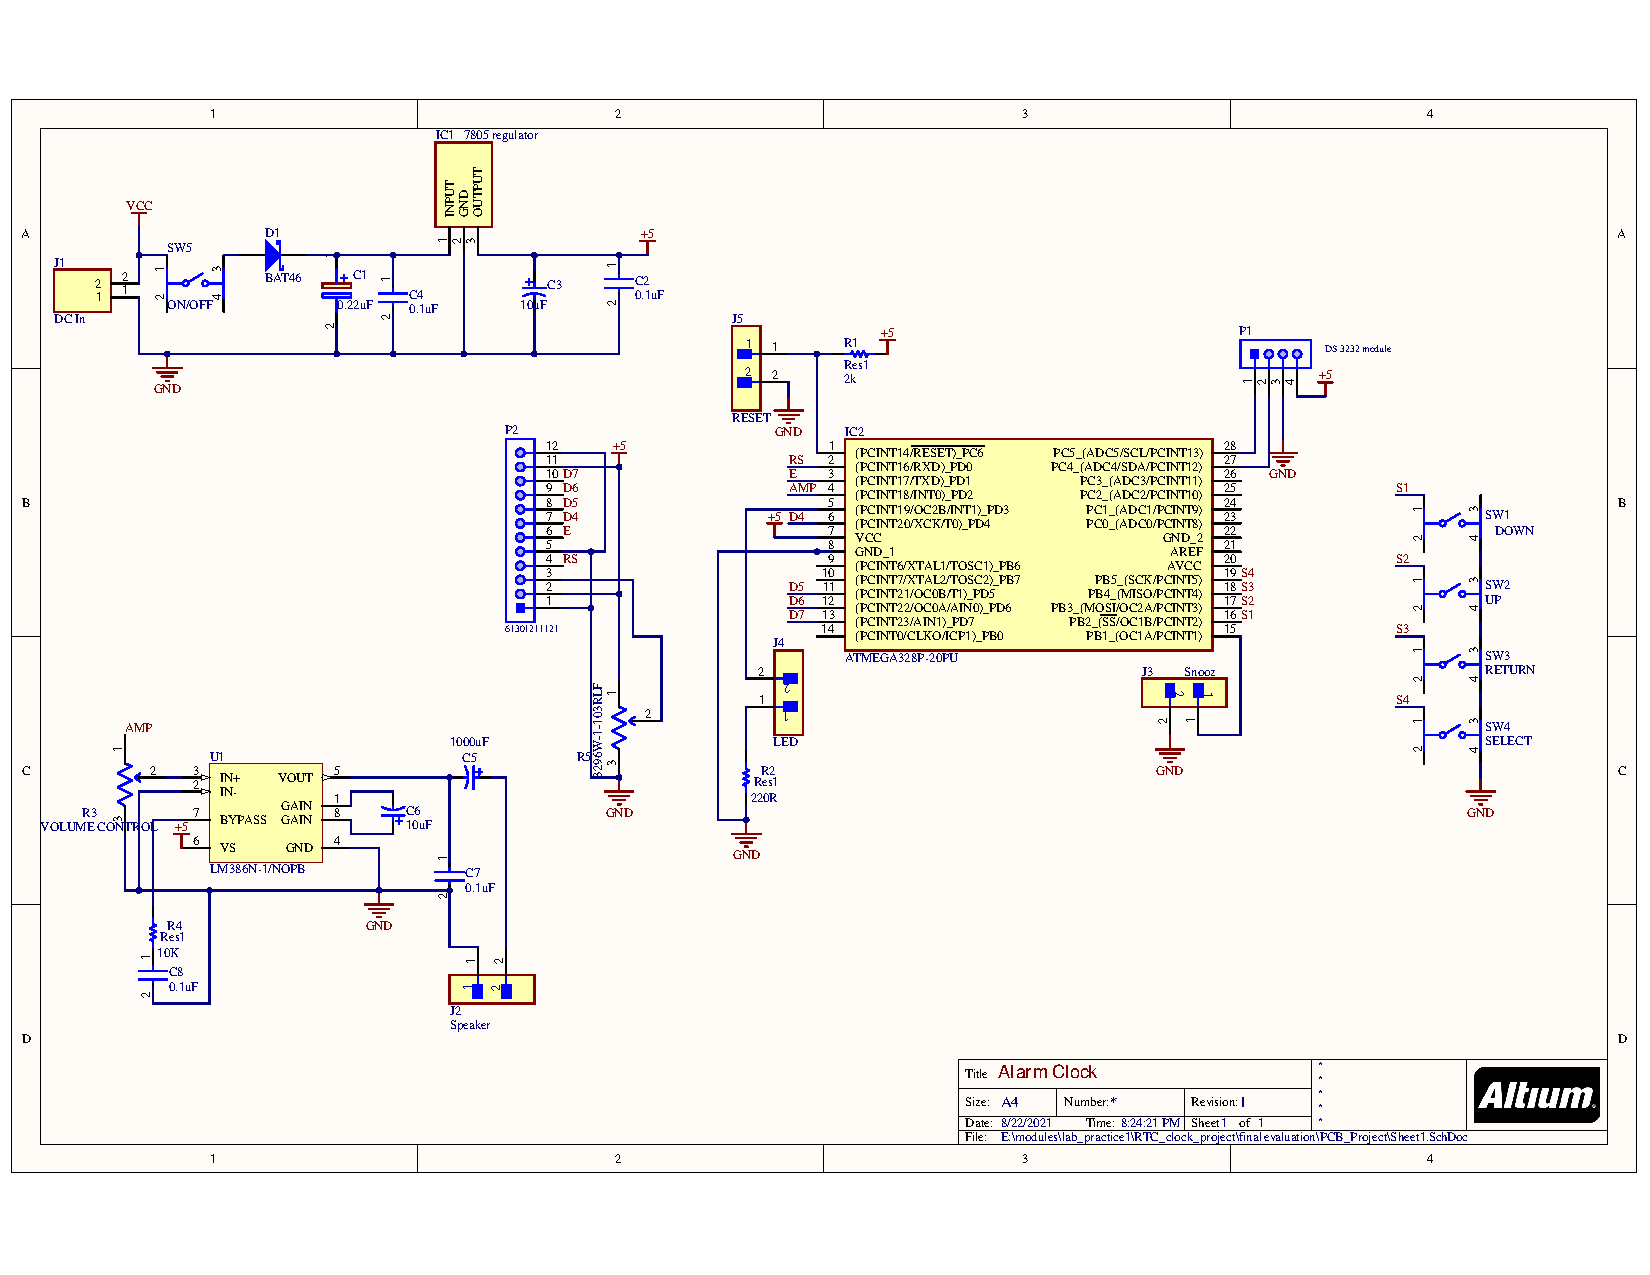
\includegraphics[width=\textwidth]{schematic.pdf}
\end{figure}
\end{center}

\newpage
\section{PCB Layout}
\begin{center}
    \begin{figure}[h]
        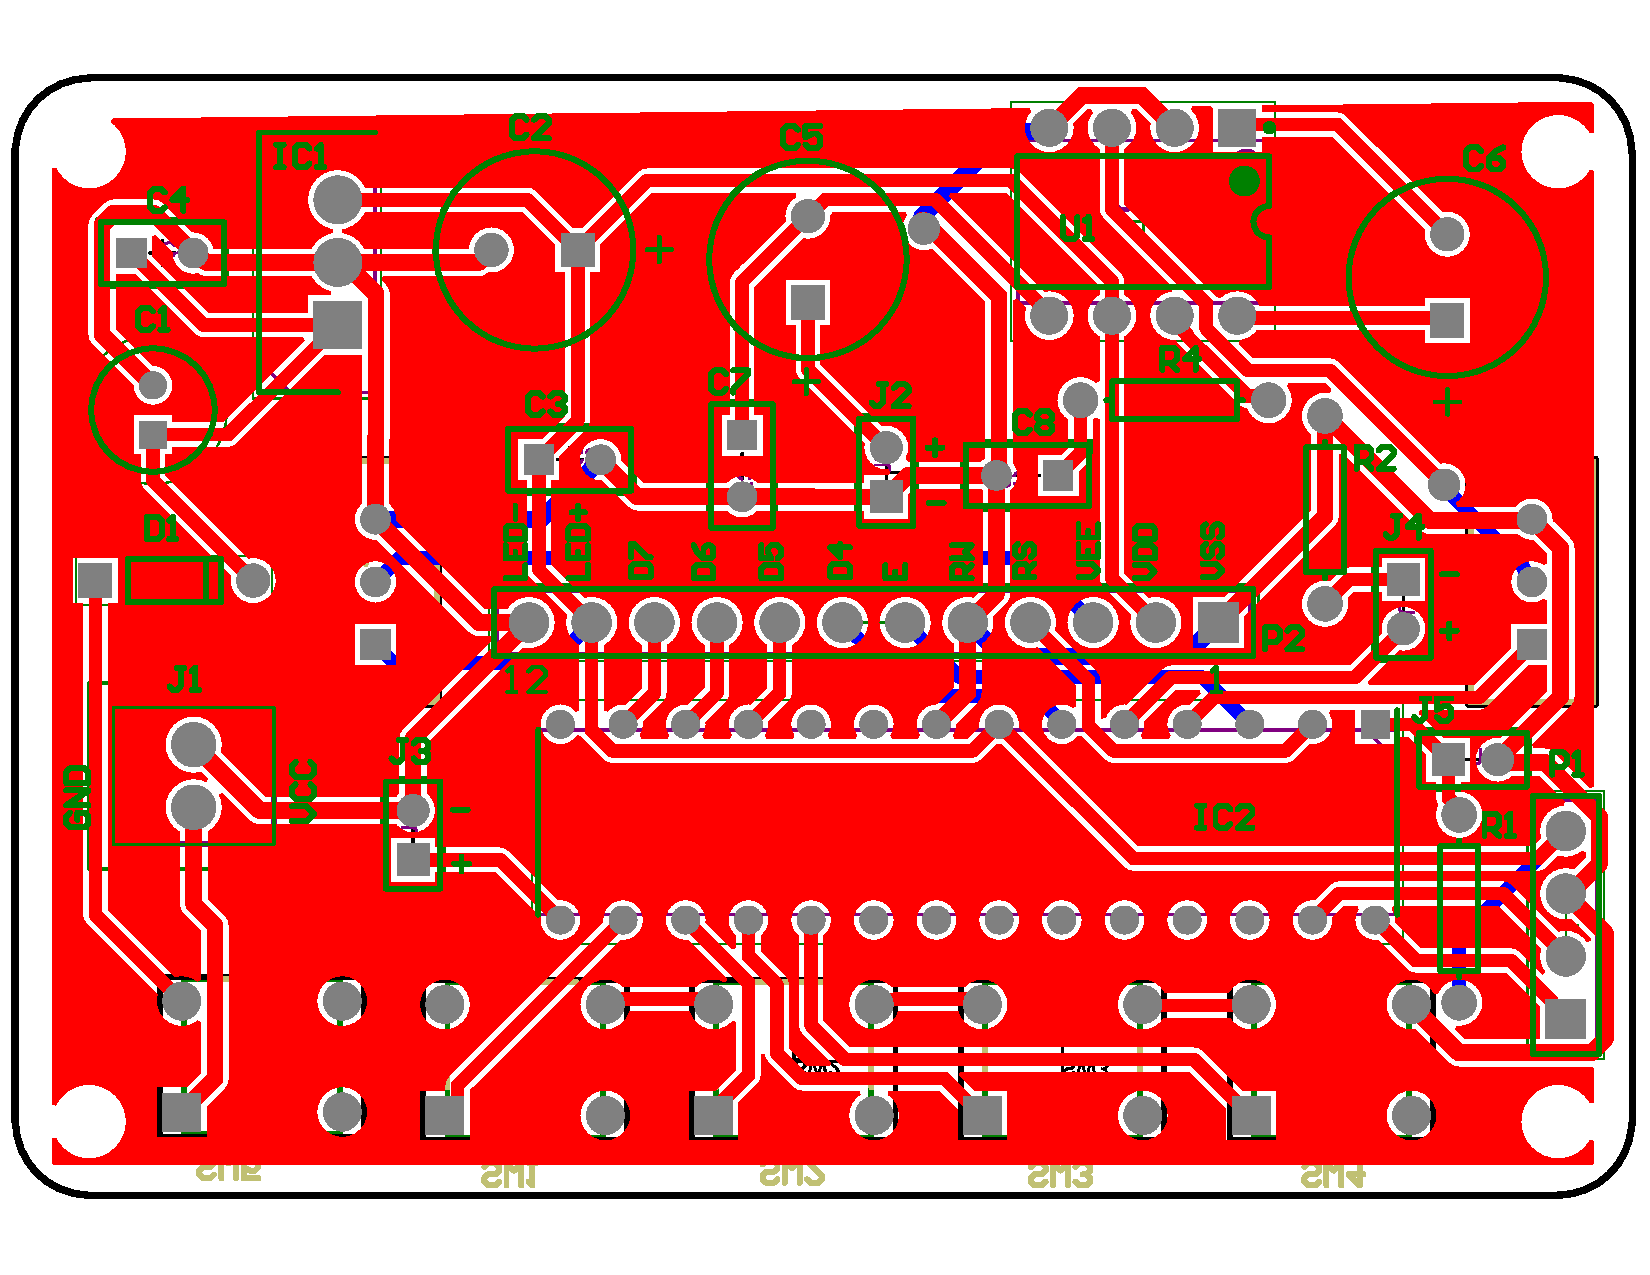
\includegraphics[width=\textwidth]{layout}
    \end{figure}
\end{center}

\begin{center}
    \begin{figure}[!h]
        \centering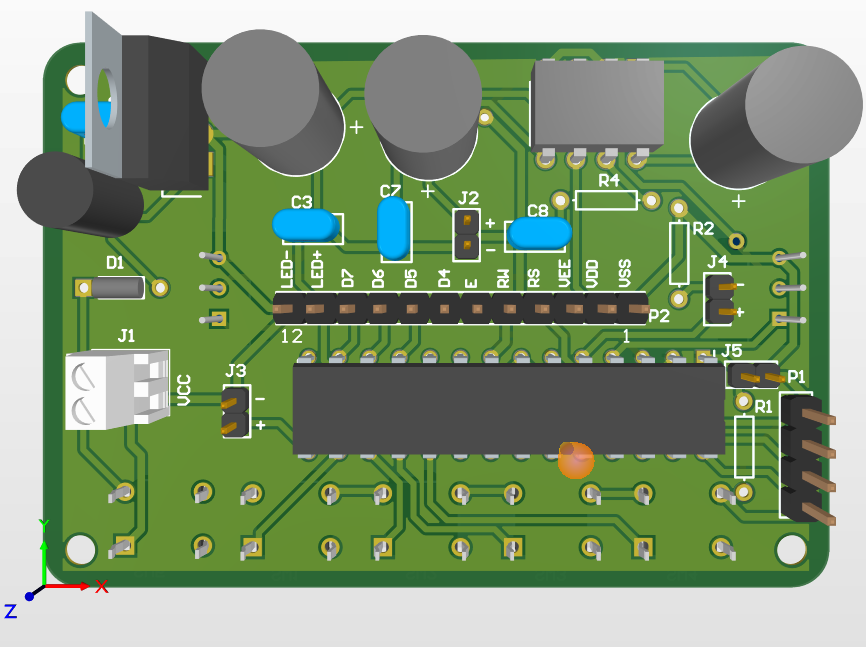
\includegraphics[width=0.70\textwidth]{front}
        \caption*{Front Side View of 3D Model}
        \centering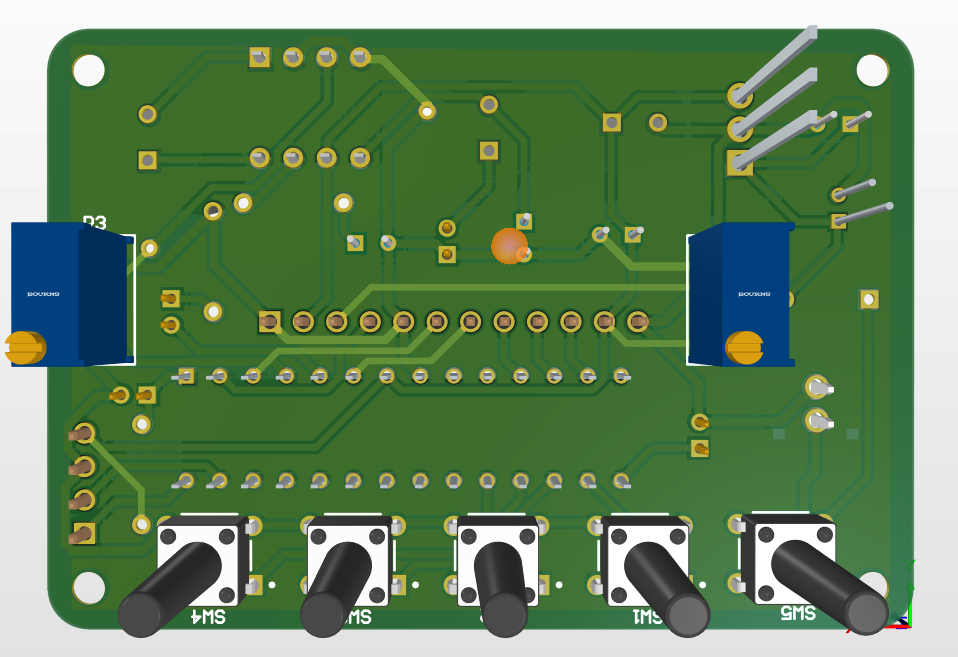
\includegraphics[width=0.70\textwidth]{back}
        \caption*{Back Side View of 3D Model}
    \end{figure}
\end{center}

\newpage
\section{Enclosure Design}
\begin{center}
    \begin{figure}[!h]
        \centering
\includegraphics[width=0.50\textwidth]{fronte}
        \caption*{Front View}
    \end{figure}
\end{center}

\begin{center}
    \begin{figure}[!h]
        \centering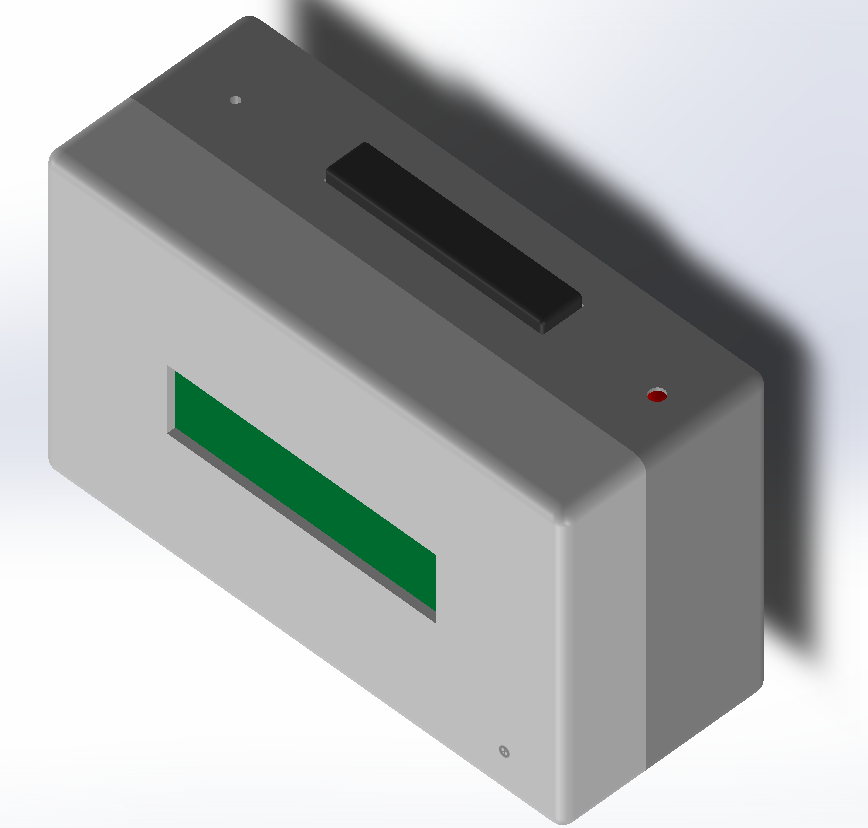
\includegraphics[width=0.50\textwidth]{tope}
        \caption*{Top View}
    \end{figure}
\end{center}

\begin{center}
    \begin{figure}[!h]
        \centering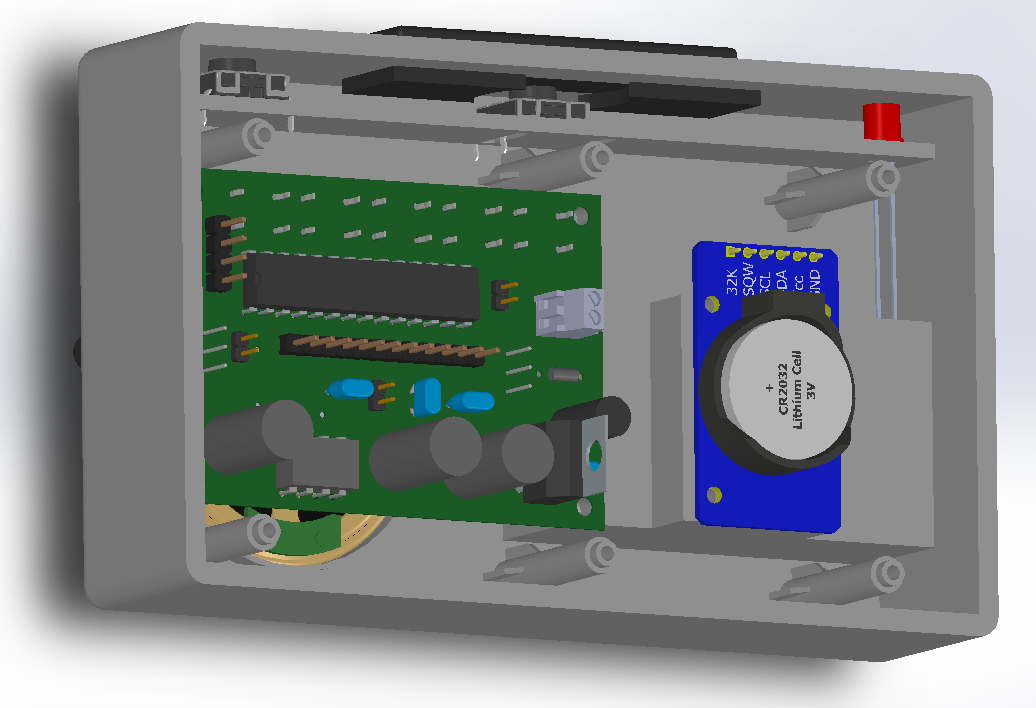
\includegraphics[width=0.60\textwidth]{backbb}
        \caption*{Inside Solid View}
    \end{figure}
\end{center}


\begin{center}
    \begin{figure}[!h]
        \centering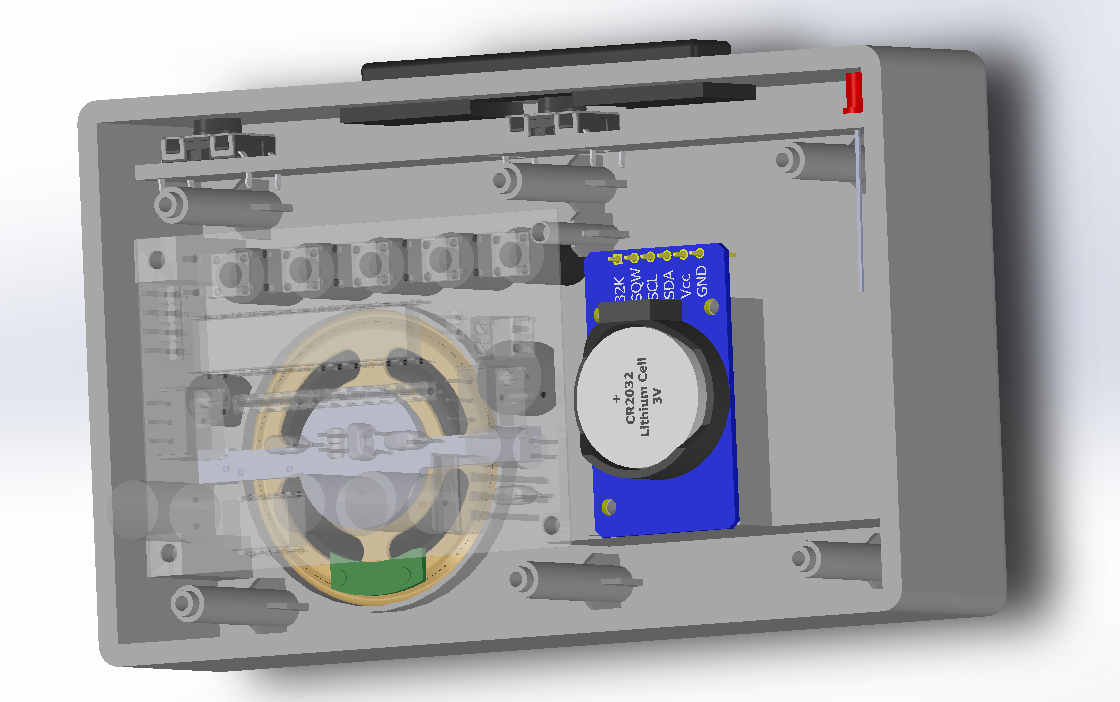
\includegraphics[width=0.60\textwidth]{backb}
        \caption*{Inside Transparent View}
    \end{figure}
\end{center}

\begin{center}
    \begin{figure}[!h]
        \centering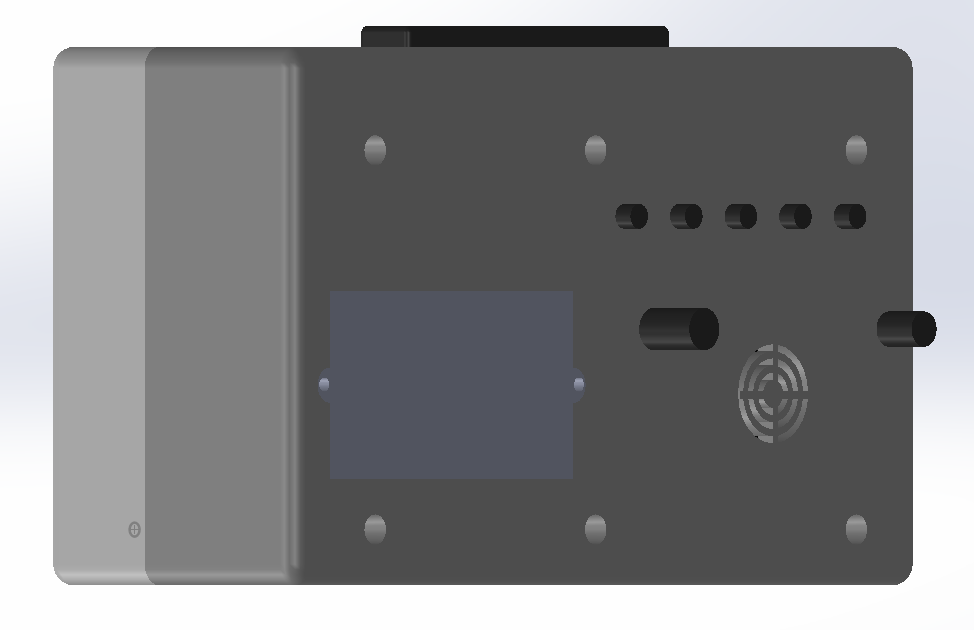
\includegraphics[width=0.60\textwidth]{backe}
        \caption*{Back View}
    \end{figure}
\end{center}

\begin{center}
    \begin{figure}[!h]
        \centering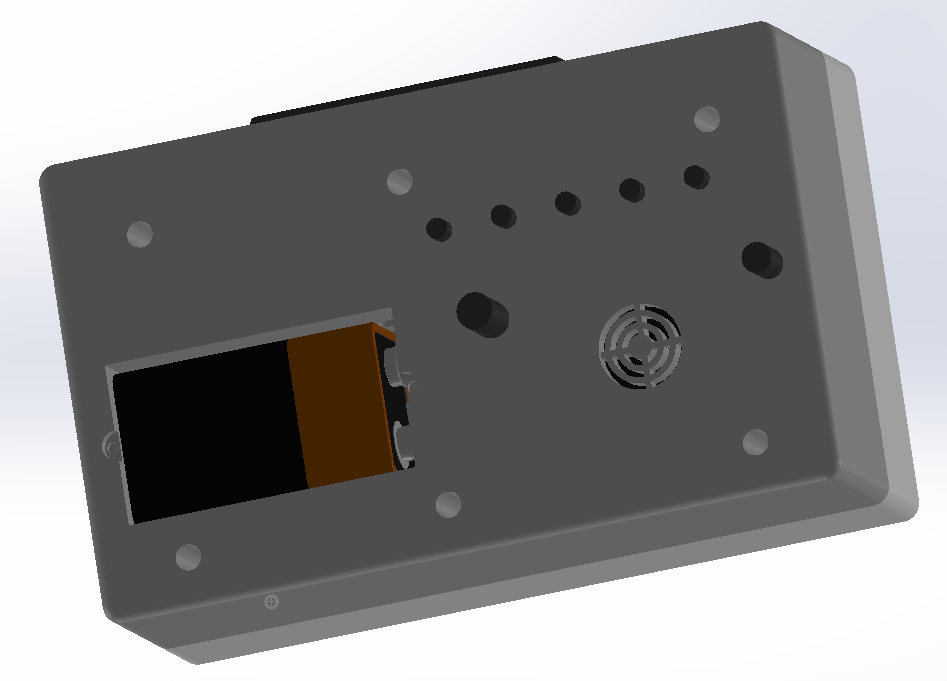
\includegraphics[width=0.60\textwidth]{battery}
        \caption*{Battery Compartment}
    \end{figure}
\end{center}
\end{document}